% \documentclass[10pt]{beamer}
\documentclass[aspectratio=169, 10pt]{beamer} % For wider width
\usepackage[
    frametitle,
    bullettoc,
    % footer,
    % minimalfooter,
    pagenumbering,
]{ocean}

\usepackage{ngntrgduc}
\usepackage{bbm} % Indicator function
\newcommand{\dps}{\displaystyle}
% \newcommand{\E}{\mathrm{E}}
\newcommand{\E}{\mathbb{E}}
\newcommand{\Var}{\mathrm{Var}}
\newcommand{\Cov}{\mathrm{Cov}}
\newcommand{\cov}{\Sigma}
\newcommand{\eps}{\varepsilon}
\newcommand{\Normal}{\mathcal{N}}

\newcommand{\der}{\mathrm{d}}

\newcommand{\NA}{\texttt{NA}}
% \newcommand{\Xobs}[1]{\ensuremath X_{\text{obs}#1}} % Highlight command

% \DeclareMathOperator{\Id}{Id}
% \DeclareMathOperator{\relu}{ReLU}
\newcommand{\relu}{ReLU}
% \operatorname{}

\newcommand{\separator}{\vspace{2ex}\hrule\vspace{2ex}}


% \setlength\parindent{0pt}   % new paragraphs will not be indented
% \setlength{\parskip}{0.4cm} % more space between paragraphs
% \setlength{\parskip}{0.25cm} % more space between paragraphs
% \setlength{\parskip}{\baselineskip} 
\setlength{\parskip}{0.2cm}
% \setlength{\parskip}{0.25cm} % more space between paragraphs
\linespread{1.25}
% \renewcommand{\baselinestretch}{1.3}

% Change the font of mathematical content to a serif font
\usefonttheme[onlymath]{serif}

% Color setup
\definecolor{red}{RGB}{219, 0, 0}

\usepackage{multirow}

\usepackage[
    backend=biber,
    % style=alphabetic,
    sorting=none,  % Entries are processed in citation order 
    % sorting=ydnt  % sort by year (descending), name, title 
]{biblatex}
\addbibresource{refs.bib}

\hypersetup{
    colorlinks,
    citecolor=magenta,
    linkcolor=black,
    urlcolor=cyan,
    pdftitle={Xử lý dữ liệu khuyết},
    pdfauthor={Trung-Duc Nguyen}
}

% Preamble ---------------------------------------------------------------
\title[xử lý dữ liệu khuyết]{\huge Xử lý dữ liệu khuyết}
\author[Nguyễn Trung Đức]{
    Nguyễn Trung Đức -- 21110269
}

\institute[HCMUS]{
    % \vspace{-.25in}
    \inst{}
    \normalsize{Khoa Toán - Tin học, Trường Đại học Khoa học Tự nhiên}
}

\graphicspath{{images/}}
\titlegraphic{
    
\includegraphics[height=2.3cm]{math-logo.png}
    \hspace{1.0cm}
    
\includegraphics[height=2.5cm]{hcmus.png}
}


% \date{\small\vspace{-.25in}\today}
\date{\small\vspace{-.25in}\today}

\addtobeamertemplate{author}{}{Giảng viên hướng dẫn: TS. Hoàng Văn Hà \par}

\setbeamertemplate{title page}{
    \vbox{}
    \vfill
    \begingroup
        \centering
        \usebeamertemplate{title}
        \vspace{1em} 
        \usebeamertemplate{author}
        % \vspace{-.25in}
        \usebeamertemplate{titlegraphic}
        % \vspace{-.25in}
        \usebeamertemplate{institute}
        \usebeamertemplate{date}
    \endgroup
    \vfill
}


\begin{document}

% Define theorems
\newtheorem{thm}{Định lý}[section]
\newtheorem{lem}{Bổ đề}[section]
\newtheorem{defi}{Định nghĩa}[section]
% \newtheorem{corollary}{Hệ quả}[section]
% \newtheorem{proof}{Chứng minh}[section]
\newtheorem{prop}{Mệnh đề}[section]
\newtheorem{assume}{Giả thiết}[section]
% \newtheorem{prop}{Mệnh đề}[section]
\newtheorem{remark}{Nhận xét}[section]
\newtheorem{ex}{Ví dụ}[section]
% \newtheorem{notation}[define]{Kí hiệu}

\numberwithin{equation}{section}
\numberwithin{figure}{section}


\begin{frame}[plain] % [Plain] hide headline and footline of the first slide
    \maketitle 
\end{frame}

\begin{frame}{Table of Contents}
    \tableofcontents[subsectionstyle=hide, subsubsectionstyle=hide]
    % \tableofcontents
\end{frame}

\section{Giới thiệu về dữ liệu khuyết}
\begin{frame}{Giới thiệu về dữ liệu khuyết}
    Dữ liệu khuyết (Missing data) là một vấn đề phổ biến trong lĩnh vực Khoa học dữ liệu, đặc biệt với các bài toán học có giám sát (supervised learning).

    Nguyên nhân: Do quá trình khảo sát không thu thập được dữ liệu, do lỗi ở phía thiết bị hoặc phần mềm thu thập dữ liệu, do quá trình xử lý dữ liệu,...

    Do đó, các dữ liệu khuyết cũng nên được chia ra theo từng loại dựa trên nguyên nhân gây ra dữ liệu bị khuyết để có cách xử lý phù hợp.
\end{frame}

\begin{frame}{Các cơ chế dữ liệu khuyết (Missing data mechanisms)}
    Cơ chế dữ liệu khuyết là các quy tắc hoặc lý do mà dữ liệu bị khuyết.
    
    Theo Donald B. Rubin (1976) \cite{rubin1976inference}, có 3 cơ chế dữ liệu khuyết:
    \begin{itemize}
        \item \textbf{MCAR (Missing Completely At Random)}: Dữ liệu bị khuyết không phụ thuộc vào dữ liệu quan sát được hoặc không quan sát được.
        \item \textbf{MAR (Missing At Random)}: Dữ liệu bị khuyết chỉ phụ thuộc vào dữ liệu quan sát được và không phụ thuộc vào dữ liệu không quan sát được (hay chính nó).
        \item \textbf{MNAR (Missing Not At Random)}: 
        % Dữ liệu bị khuyết phụ thuộc vào dữ liệu quan sát được và không quan sát được, hoặc chỉ phụ thuộc vào dữ liệu dữ liệu không quan sát được, hay chính nó.
        Dữ liệu bị khuyết phụ thuộc vào chính giá trị bị khuyết hoặc các giá trị không quan sát được.
    \end{itemize}
\end{frame}


\begin{frame}{Xử lý dữ liệu khuyết}
    Thông thường, có 3 hướng tiếp cận:
    \begin{itemize}
        \item Loại bỏ toàn bộ các dữ liệu bị khuyết (Listwise deletion).
        
        \item Điền khuyết (Impute) dữ liệu bằng các phương pháp điền khuyết.
        
        \item Sử dụng các phương pháp có thể tự xử lý dữ liệu khuyết.
    \end{itemize}    
\end{frame}

\section{Giới thiệu bài toán}
\begin{frame}{Giới thiệu bài toán}
    Bài toán hồi quy tuyến tính với dữ liệu khuyết.

    \begin{itemize}
        \item Trong thực tế, ta không thể biết được dữ liệu bị khuyết theo cơ chế nào nếu chỉ dựa vào dữ liệu.
        \item Đa số các hướng tiếp cận đều giả sử với cơ chế MCAR hay MAR.
        \item Ta muốn phương pháp phải mạnh (robust) với từng loại cơ chế khác nhau.
    \end{itemize}
    \pause
    $\Rightarrow$ Bài báo \cite{le2020neumiss} đề xuất phương pháp xấp xỉ bằng chuỗi Neumann cho dự đoán Bayes (dự đoán tối ưu nhất), dưới những giả định cơ chế dữ liệu khuyết khác nhau, cho ra kết quả chính xác, hiệu quả và ổn định hơn so với lại các phương pháp khác.

    % Trong thực tế, các nhà phân tích dữ liệu thường phải giả sử 1 trong 3 loại cơ chế dữ liệu khuyết vì họ không biết rằng dữ liệu bị khuyết thực tế sẽ thuộc vào kiểu cơ chế nào. Bài báo đề xuất một mô hình có thể xử lý đồng thời cả 3 loại cơ chế trong bài toán hồi quy tuyến tính, mà không cần các bước điền khuyết truyền thống.
\end{frame}

\begin{frame}{Một số ký hiệu}
    \begin{columns}
    \column{0.5\textwidth}
    Ký hiệu:
    \begin{itemize}
        \item $X \in \R^d$: Dữ liệu đầy đủ
        \item $\widetilde{X} \in \{\R \cup \{\NA\}\}^d$: Dữ liệu bị khuyết
        \item $M \in \{0, 1\}^d$: Vector mask
    \end{itemize}
    
    Với mọi $1 \leq j \leq d:$
    \begin{align*}
        M_j &= 
        \begin{cases}
            1, \ \text{nếu } X_j \text{ bị khuyết} \\
            0, \ \text{nếu } X_j \text{ không bị khuyết}
        \end{cases}\\
        \widetilde{X}_j &= 
        \begin{cases}
        \NA, \text{ nếu } M_j = 1 \\
        X_j, \text{ nếu } M_j = 0
        \end{cases}
    \end{align*}
    
    \column{0.5\textwidth}
    Ví dụ:
    \[
        \begin{split}
            x &= (1.1, 2.2, -3.5, 4, 5.6) \\
            \widetilde{x} &= (1.1, \NA, -3.5, 4, \NA) \\
            m &= (0, 1, 0, 0, 1) \\
            % obs(m) &= (0, 2, 3) \\
            x_{obs(m)} &= (1.1, -3.5, 4) \\
            % mis(m) &= (1, 4) \\
            x_{mis(m)} &= (2.2, 5.6) \\
        \end{split}
    \]
    \end{columns}

\end{frame}

\begin{frame}{Mô hình bài toán}
    Ta xét mô hình hồi quy tuyến tính tổng quát với các biến độc lập $X_1, X_2, \dots, X_d \in \R$, biến phụ thuộc $Y \in \R$, hệ số hồi quy $\beta_0, \beta_1, \dots, \beta_d$, và sai số ngẫu nhiên $\eps \sim \Normal(0, \sigma^2)$:
    \begin{align*}
        Y 
        &= \beta_0 + \beta_1 X_1  + \beta_2 X_2 + \dots + \beta_d X_d + \eps \\
        &= \beta_0 +  \sum_{j=1}^d \beta_j X_j + \eps \\
        &= \beta_0 + \langle X, \beta \rangle + \eps.    
    \end{align*}
    với $\beta = (\beta_1, \beta_2, \dots, \beta_d) \in \R^d$, $X = (X_1, X_2, \dots, X_d) \in \R^d$, và $\langle \cdot, \cdot \rangle$ là tích vô hướng.
    
\end{frame}

\section{Dự đoán Bayes (Bayes predictor)}
\begin{frame}{Dự đoán Bayes (Bayes predictor)}

    Giả sử quá trình sinh dữ liệu của $Y$ được xác định bởi mô hình hồi quy tuyến tính cho dữ liệu đầy đủ $X$ như sau:
    \begin{equation*}\label{eq:lr_matrix_notation}
        Y = \beta_0^* + \langle X, \beta^* \rangle + \eps,
    \end{equation*}
    với $\beta_0^*$, $\beta^* = (\beta_1^*, \beta_2^*, \dots, \beta_d^*)$ là các hệ số chính xác (true coefficients) để xây dựng mô hình.
    
    
    \pause
    Sẽ khó để ước lượng các hệ số hồi quy khi dữ liệu bị khuyết, đặc biệt là khi $d$ lớn, hay với các mẫu (pattern) dữ liệu khuyết phức tạp theo $m$.
    \pause
    
    Thay vào đó, ta sẽ tìm một hàm $f$ mà nó ánh xạ dữ liệu 
    bị khuyết $\widetilde{X}$ 
    thành giá trị $Y$, hay $f$ là mô hình đưa ra dự đoán dựa trên dữ liệu 
    bị khuyết $\widetilde{X}$.

    \pause
    Ta có dự đoán Bayes (dự đoán tối ưu):
    \[
        f_{\widetilde{X}}^* \in \argmin_{f: \widetilde{\mathcal{X}} \to \R} \E [(Y - f(\widetilde{X}))^2].
    \]
\end{frame}

\begin{frame}{Dự đoán Bayes (Bayes predictor)}
    Do $\widetilde{X}$ tồn tại những phần tử $\NA$ đại diện cho dữ liệu khuyết, nên ta khó có thể tính toán $f$.
    Ta viết lại dự đoán Bayes dưới dạng
    một hàm của dữ liệu quan sát được $X_{\text{obs}(M)}$ và vector mask $M$:
    \begin{equation*}
        \begin{split}
        f^* (X_{obs(M)}, M) 
        &= \E [Y | M, X_{\text{obs}(M)}] \\
        &= \E [\beta_0^* + \langle \beta^*, X \rangle | M, X_{obs(M)}] \\
        &= \beta_0^* + \E [\langle \beta_{obs(M)}^*, X_{obs(M)} \rangle | M , X_{obs(M)}] + \E [\langle \beta_{mis(M)}^*, X_{mis(M)} \rangle | M , X_{obs(M)}] \\
        &= \beta_{0}^{*} + \langle\beta_{obs(M)}^{*}, X_{obs(M)}\rangle 
        + \langle\beta_{mis(M)}^{*}, \E [X_{mis(M)} | M, X_{obs(M)}] \rangle. 
        \end{split} 
    \end{equation*} 
    với $\beta_{obs(M)}^{*}$, $\beta_{mis(M)}^{*}$ tương ứng với hệ số hồi quy của các phần tử không bị khuyết và bị khuyết.
    
    \pause
    Khó để biểu diễn dự đoán Bayes dưới dạng đóng (closed-form) 
    vì nó phụ thuộc vào phân phối của dữ liệu, cũng như đặc điểm riêng của từng cơ chế.
    
    \pause
    Dẫu vậy, với dữ liệu $X$ tuân theo phân phối chuẩn đa biến: $X \sim \Normal(\mu, \cov)$, ta vẫn có thể biểu diễn dự đoán Bayes dưới dạng đóng cho từng loại cơ chế cụ thể. 
\end{frame}


\subsection{Dự đoán Bayes cho cơ chế M(C)AR}
\begin{frame}{Dự đoán Bayes cho cơ chế M(C)AR}
    
    \only<1>{Dự đoán Bayes tổng quát có dạng:}
    \[
        f^* (X_{obs(M)}, M) = \beta_{0}^{*} + \langle\beta_{obs(M)}^{*}, X_{obs(M)}\rangle 
    + \langle\beta_{mis(M)}^{*}, {\E [X_{mis(M)} | M, X_{obs(M)}]} \rangle.
    \]

    \pause
    Với mọi $m \in \{0, 1\}^d$, ta có
    \vspace{0.5em}
    \begin{columns}
        \column{0.4\textwidth}
        \textbf{Giả thiết cơ chế MCAR}
        \begin{equation*}
            P(M = m | X) = P(M = m).    
        \end{equation*}

        \column{0.4\textwidth}
        \textbf{Giả thiết cơ chế MAR}: 
        \begin{equation*}
            P(M = m | X) = P(M = m | X_{obs(m)}).
        \end{equation*}
    \end{columns}

    \pause

    \begin{prop}[Dự đoán Bayes với M(C)AR]
    Giả sử dữ liệu được sinh ra từ mô hình tuyến tính và có phân phối chuẩn đa biến. Giả sử ta có giả thiết cơ chế MCAR hoặc MAR, thì dự đoán Bayes $f^*$ có dạng:
    \begin{equation*}\label{eq:mcar_bayes_predictor}
        f^* (X_{obs},M ) =
        \beta_{0}^{*} + \langle\beta_{obs}^{*},X_{obs} \rangle+\langle\beta_{mis}^{*},\mu_{mis} + \cov_{mis,obs}(\cov_{obs})^{-1}(X_{obs}-\mu_{obs})\rangle.
    \end{equation*}
\end{prop}
\end{frame}



\subsection{Dự đoán Bayes cho cơ chế MNAR}
\begin{frame}{Dự đoán Bayes cho cơ chế MNAR}
    \textbf{Khó khăn:} 
    Với MNAR, dữ liệu bị khuyết phụ thuộc vào chính giá trị bị khuyết hoặc các giá trị không quan sát được, nên sẽ khó để mô hình hoá.

    \pause
    \textbf{Giả thiết Gaussian self-masking}
    Cơ chế dữ liệu bị khuyết được gọi là self-masked với 
    $P(M|X) = \dps\prod_{k=1}^d P(M_k|X_k)$ và $\forall k \in [1,d]$,
    \[
        P(M_{k} = 1 | X_{k}) = K_{k} \exp\left( -\frac{1}{2} \frac{(X_{k} - \widetilde{\mu}_{k})^{2}}{\widetilde{\sigma}_{k}^{2}} \right), \quad \text{ với } 0 < K_{k} < 1.
    \]
    \begin{itemize}
        \item $K_k$ là hằng số điều chỉnh xác suất $X_k$ bị khuyết.
        \item Xác suất để $X_k$ bị khuyết không phụ thuộc vào các giá trị khác.
        \item Xác suất để $X_k$ bị khuyết 
        % ($M_k = 1$) phụ thuộc vào chính $X_k$
        tuân theo phân phối chuẩn $\Normal(\widetilde{\mu}_{k}, \widetilde{\sigma}_{k}^2 )$.
    \end{itemize}
\end{frame}

\begin{frame}{Dự đoán Bayes cho cơ chế MNAR}
    \begin{prop}[Dự đoán Bayes với Gaussian self-masking]
    Giả sử dữ liệu được sinh ra từ mô hình tuyến tính, tuân theo phân phối chuẩn đa biến và thoả giả thiết Gaussian self-masking. 
    Cho $\cov_{mis|obs} = \cov_{mis,mis} - \cov_{mis,obs} (\cov_{obs})^{-1} \cov_{obs,mis}$,
    và $D$ là ma trận đường chéo sao cho $\diag(D) = (\sigma_1^2, \dots, \sigma_d^2)$. Lúc này, dự đoán Bayes được viết dưới dạng:
    \begin{multline*}\label{eq:gaussian_bayes_predictor}
        f^{*}(X_{obs}, M) = 
        \beta_{0}^{*} + \langle\beta_{obs}^{*}, X_{obs}\rangle 
        + \langle\beta_{mis}^{*},(Id + D_{mis} \cov_{mis|obs}^{-1})^{-1} \\
        \times (\tilde{\mu}_{mis} + D_{mis}\cov_{mis|obs}^{-1}(\mu_{mis} + 
        \cov_{mis,obs}\left(\cov_{obs}\right)^{-1} (X_{obs}-\mu_{obs}))) \rangle.
    \end{multline*}
    \end{prop}
\end{frame}

\subsection{Dự đoán Bayes cho các cơ chế dữ liệu khuyết}
\begin{frame}{Dự đoán Bayes cho các cơ chế dữ liệu khuyết}
    Trường hợp M(C)AR:
    \[
        f^* (X_{obs},M ) =
        \beta_{0}^{*} + \langle\beta_{obs}^{*},X_{obs} \rangle+\langle\beta_{mis}^{*},\mu_{mis} + \cov_{mis,obs} \textcolor<2>{red}{(\cov_{obs})^{-1}}(X_{obs}-\mu_{obs})\rangle.
    \]
    
    Trường hợp MNAR:
    \begin{multline*}
        f^{*}(X_{obs}, M) = 
    \beta_{0}^{*} + \langle\beta_{obs}^{*}, X_{obs}\rangle 
    + \langle\beta_{mis}^{*},(Id + D_{mis} \cov_{mis|obs}^{-1})^{-1} \\
    \times (\tilde{\mu}_{mis} + D_{mis}\cov_{mis|obs}^{-1}(\mu_{mis} + 
    \cov_{mis,obs}\textcolor<2>{red}{\left(\cov_{obs}\right)^{-1}} (X_{obs}-\mu_{obs}))) \rangle.
    \end{multline*}
    \pause
    % \only<2>
    {\textbf{Khó khăn:} Khi $d$ lớn thì chi phí tính toán cho $(\cov_{obs})^{-1}$ sẽ rất lớn.}
\end{frame}


\section{Mạng NeuMiss}
\begin{frame}{Xấp xỉ dự đoán Bayes bằng chuỗi Neumann}
    Chuỗi Neumann cho ma trận $A$ được định nghĩa như sau:
    \[
        \sum_{k=0}^{\infty} A^k = I + A + A^2 + \dots,
    \]
    và khi chuỗi hội tụ ($\|A\|_2 < 1$), tồn tại nghịch đảo của $(I - A)$ với:
    \[
        (I - A)^{-1} = \sum_{k=0}^{\infty} A^k.
    \]
    Từ đây, chuỗi Neumann có thể được sử dụng để xấp xỉ nghịch đảo của một ma trận: Xét ma trận $A$ khả nghịch, ta có:
    \[
        A^{-1} = (I - (I - A))^{-1} = \sum_{k=0}^{\infty} (I - A)^k.
    \]
\end{frame}


\begin{frame}{Xấp xỉ dự đoán Bayes bằng chuỗi Neumann}
    Xấp xỉ bằng chuỗi Neumann dưới dạng phép lặp:
    \begin{equation*}\label{eq:iterative_fomula}
        S_{obs(m)}^{(\ell)} = (Id - \cov_{obs(m)}) S_{obs(m)}^{(\ell - 1)} + Id.
    \end{equation*}

    \begin{prop}[Hội tụ tuyến tính của phép lặp Neumann]
        Giả sử $\|\cov\|_2 < 1$. Với mọi $m \in \{0,1\}^d$, phép lặp $S^{(\ell)}_{obs(m)}$ hội tụ tuyến tính về $(\cov_{obs(m)})^{-1}$ và thoả mãn với mọi $\ell \geq 1$,
        với $\nu_{obs(m)}$ là trị riêng nhỏ nhất của $\cov_{obs(m)}$,
        \begin{equation*}\label{eq:iteration_converge_bound}
        \|Id - \cov_{obs(m)} S_{obs(m)}^{\ell}\|_2 
        \leq (1 - \nu_{obs(m)})^{\ell} \|Id - \cov_{obs(m)} S_{obs(m)}^{(0)}\|_2.
        \end{equation*}
    \end{prop}
\end{frame}

\section*{Kết quả thực nghiệm}
\begin{frame}{Kết quả thực nghiệm: Xấp xỉ ma trận bằng chuỗi Neumann}
    \begin{figure}[h]
        \centering
        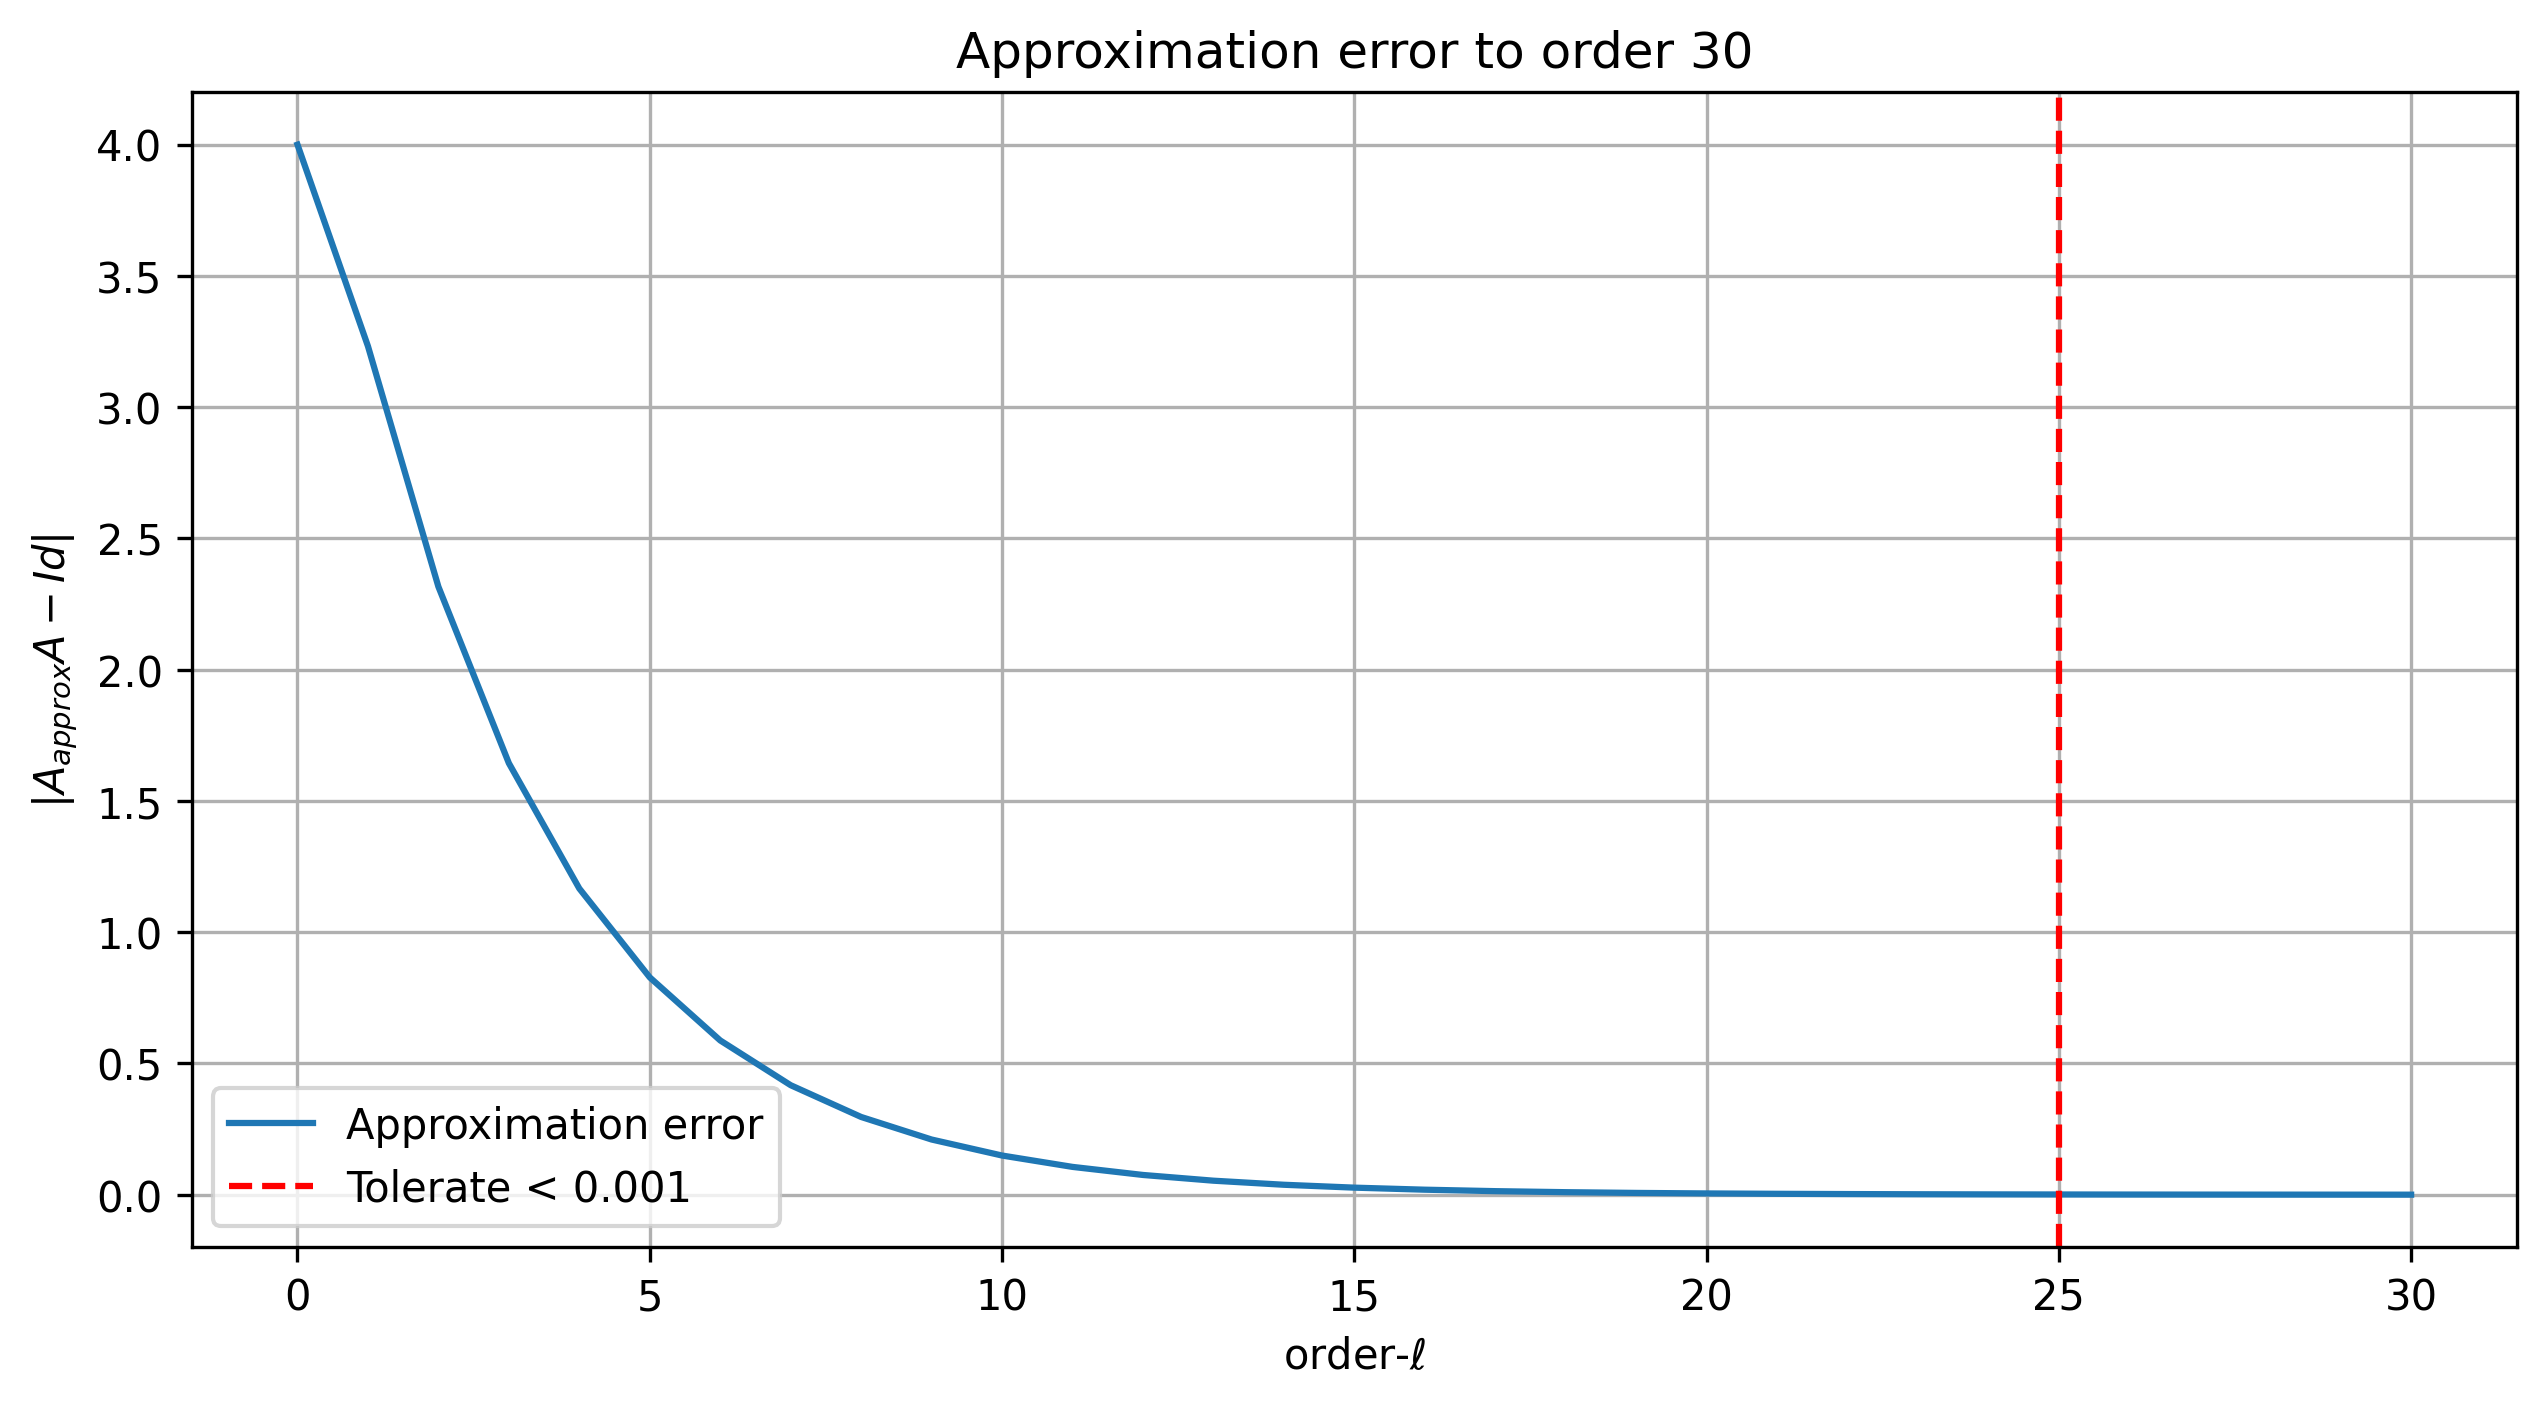
\includegraphics[width=.8\textwidth]{approx_neumann.png}
        \caption{
            Sai số của xấp xỉ ma trận tới bậc $30$.
        }
    \end{figure}
\end{frame}

\begin{frame}{Xấp xỉ dự đoán Bayes bằng chuỗi Neumann}

    Ta có xấp xỉ bậc-$\ell$ của dự đoán Bayes trong trường hợp cơ chế M(C)AR dưới dạng:
    \begin{equation*}\label{eq:l_approximation_mcar_bayes_predictor}
        f_{\ell}^* (X_{obs}, M) = \langle\beta_{obs}^{*},X_{obs} \rangle+\langle\beta_{mis}^{*},\mu_{mis} + \cov_{mis,obs} \textcolor{blue}{S_{obs(m)}^{(\ell)}} (X_{obs}-\mu_{obs})\rangle.
    \end{equation*}
    
    % Sai số giữa dự đoán Bayes và xấp xỉ bậc-$\ell$ của nó được cho bởi mệnh đề sau:
    \begin{prop}[Sai số giữa dự đoán Bayes và xấp xỉ bậc-$\ell$ của nó]\label{prop:error_approximation}
       Cho $\nu$ là trị riêng nhỏ nhất của $\cov$. Giả sử dữ liệu được sinh ra qua mô hình tuyến tính, tuân theo phân phối chuẩn đa biến, giả thiết MCAR hay MAR thoả, và $\|\cov\|_2 < 1$. Thì với mọi $\ell \geq 1$,
       \begin{equation*}\label{eq:aprrox_error}
           \E \left[\left(f_{\ell}^* (X_{obs}, M) - f^* (X_{obs}, M)\right)^2\right] 
           \leq \dfrac{(1-\nu)^{2\ell} \|\beta^*\|_2^2}{\nu} \ \E\left[ \|Id - S_{obs(M)}^{(0)} \cov_{obs(M)}\|_2^2\right].
       \end{equation*}
    \end{prop}
\end{frame}


\begin{frame}{Algorithm Unrolling}
    \begin{figure}
        \centering
        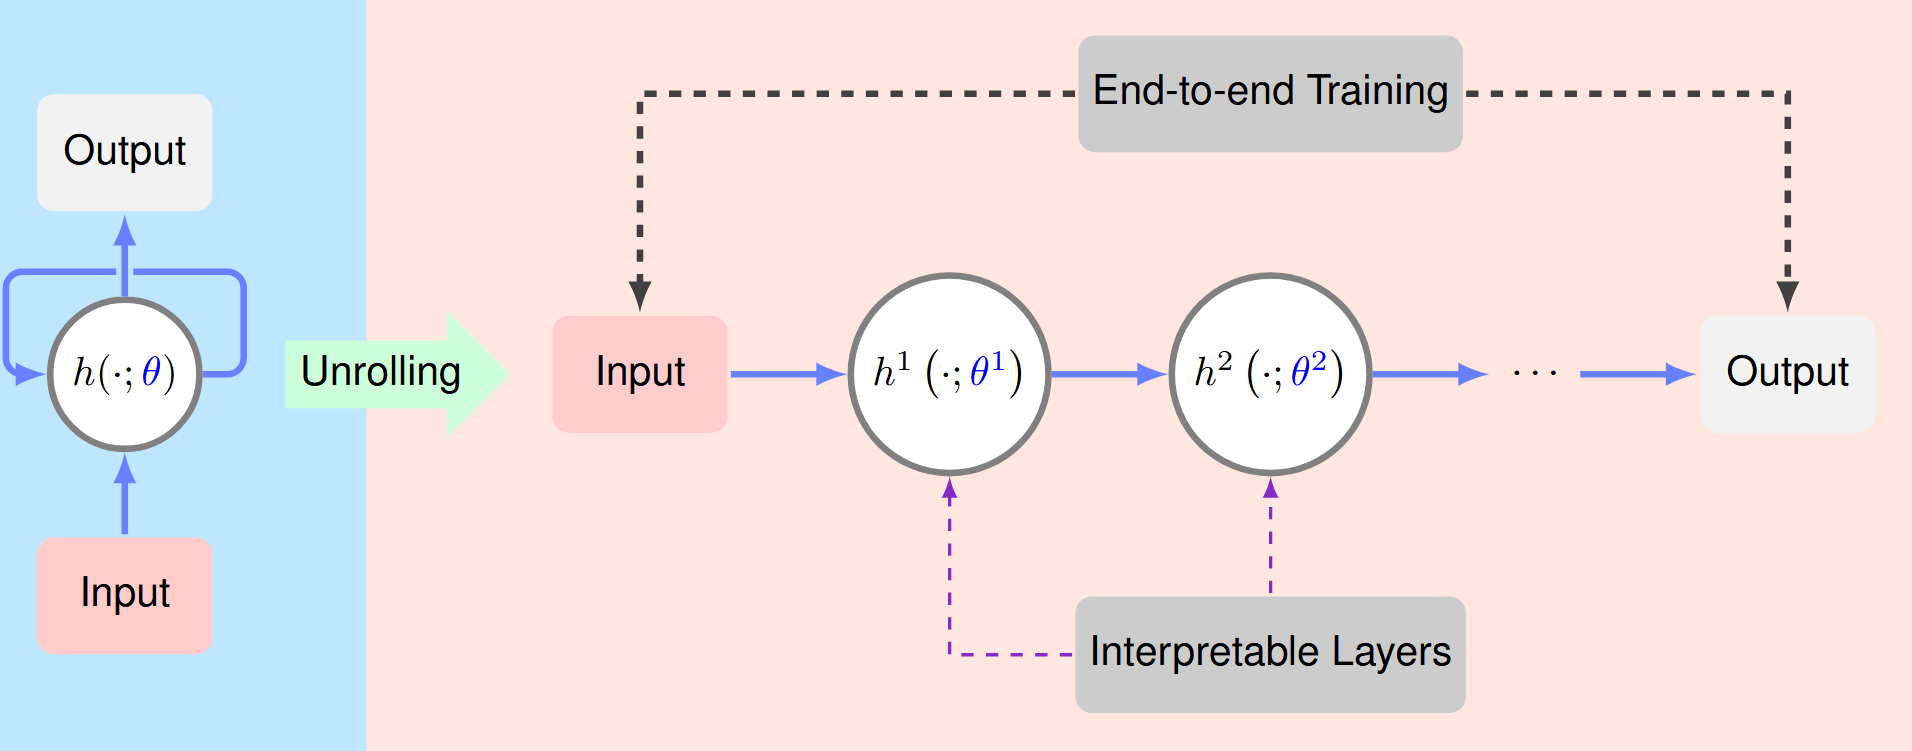
\includegraphics[width=0.9\linewidth]{unrolling.png}
        \caption{Ý tưởng Algorithm Unrolling \cite{gregor2010unroll}: Thuật toán lặp trở thành Neural network (ảnh được trích từ \cite{monga2021unroll})}
        \label{fig:algorithm-unrolling}
    \end{figure}
\end{frame}


\begin{frame}{Mạng NeuMiss}
    \begin{equation*}\label{eq:l_approximation_mcar_bayes_predictor}
        f_{\ell}^* (X_{obs}, M) = \langle {\beta_{obs}^{*}}, X_{obs} \rangle + \langle {\beta_{mis}^{*}}, \mu_{mis} + {\cov_{mis,obs}} \textcolor{blue}{S_{obs(m)}^{(\ell)}} (X_{obs}-\mu_{obs})\rangle.
    \end{equation*}
    \hrule
    \begin{figure}
        \centering
        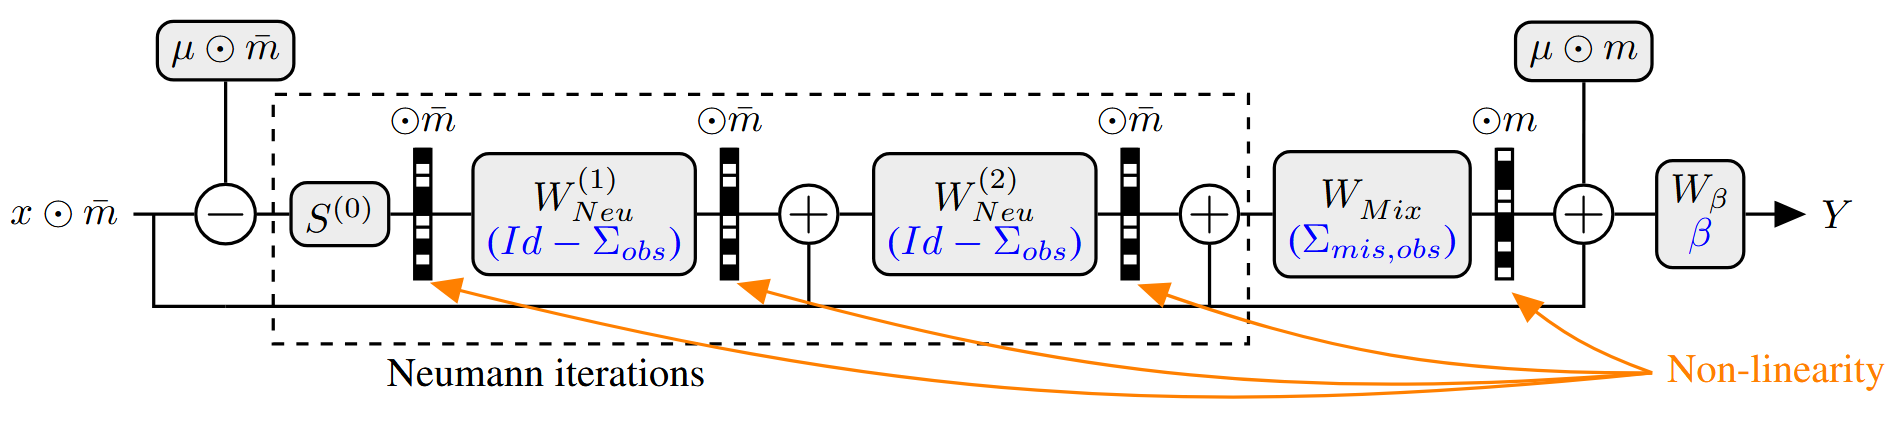
\includegraphics[width=\linewidth]{neumiss_network.png}
        \caption{Mạng NeuMiss độ sâu 4 -- $\bar{m} = 1 - m$}
        \label{fig:neumiss}
    \end{figure}    
\end{frame}

\begin{frame}{Mạng NeuMiss: Xấp xỉ cho cơ chế MNAR}
    Dự đoán Bayes với cơ chế M(C)AR:
    \[
        f^* (X_{obs},M ) =
        \beta_{0}^{*} + \langle\beta_{obs}^{*},X_{obs} \rangle+\langle\beta_{mis}^{*},\textcolor{blue}{\mu_{mis}} + \textcolor{red}{\cov_{mis,obs}} {(\cov_{obs})^{-1}}(X_{obs}-\mu_{obs})\rangle.
    \]
    % \hrule
    Giả sử $D_{mis} \cov_{mis|obs}^{-1} \approx Id$, thì dự đoán Bayes cho self-masking trở thành:
    \begin{align*}
        f^*(X_{obs}, M) 
        &\approx \beta_0^* + \langle \beta_{obs}^*, X_{obs}\rangle + \langle \beta_{mis}^*, \textcolor{blue}{\frac{1}{2} (\widetilde{\mu}_{mis} + \mu_{mis})} + \textcolor{red}{\frac{1}{2}  \cov_{mis,obs}} (\cov_{obs})^{-1} (X_{obs} - \mu_{obs}) \rangle,
    \end{align*}
    hoặc khi $D_{mis} \cov_{mis|obs}^{-1} \approx \hat{D}_{mis}$ với $\hat{D}$ là một ma trận ma trận đường chéo:
    \begin{multline*}
        f^*(X_{obs}, M) 
        \approx \beta_0^* + \langle \beta_{obs}^*, X_{obs}\rangle + \langle \beta_{mis}^*, 
        \textcolor{blue}{(Id + \hat{D}_{mis})^{-1} (\widetilde{\mu}_{mis} + \hat{D}_{mis} \mu_{mis})} \\
        + \textcolor{red}{(Id + \hat{D}_{mis})^{-1} \hat{D}_{mis} \cov_{mis,obs}} (\cov_{obs})^{-1} (X_{obs} - \mu_{obs}) \rangle.
    \end{multline*}
\end{frame}


\begin{frame}{Kết quả thực nghiệm: Mạng NeuMiss}
% Tập dữ liệu được sinh ra từ phân phối chuẩn đa biến, với $Y$ được tính bằng hàm tuyến tính của $X$, cùng với $50\%$ dữ liệu bị khuyết ngẫu nhiên (MCAR) ở mỗi đặc trưng trong tập dữ liệu và nhiễu $\varepsilon$ tuân theo phân phối chuẩn với tỷ lệ signal-to-noise (SNR) bằng~$10$.
% (tỷ lệ nhiễu nhỏ hơn $10$ lần so với ``tín hiệu'' $Y$).

% Ta sử dụng metric $R$ bình phương ($R^2$), để tính tỷ lệ của độ biến thiên cho biến phụ thuộc $Y$ được giải thích bởi biến độc lập $X$, từ đó đánh giá độ hiệu quả của mô hình. 
    \begin{table}[h!]
    \centering
    \setlength{\tabcolsep}{10pt}
    \begin{tabular}{lcccccc}
    \toprule
    & \multicolumn{2}{c}{\textbf{Train Set}} & \multicolumn{2}{c}{\textbf{Validation Set}} & \multicolumn{2}{c}{\textbf{Test Set}} \\
    \cmidrule(lr){2-3}\cmidrule(lr){4-5}\cmidrule(lr){6-7}
     & $R^2$ & MSE & $R^2$ & MSE & $R^2$ & MSE \\
    \midrule
    NeuMiss depth-10 & 0.8072 & 0.208 & 0.7482 & 0.2808 & 0.7578 & 0.2674 \\
    \bottomrule
    \end{tabular}
    % \captionsetup{justification=centering, width=\linewidth}
    \caption{Hiệu suất của NeuMiss với độ sâu 10.}
    \label{tab:performance}
    \end{table}
Với Bayes rate cho tập train là 0.8205 và tập test là 0.8078.
\end{frame}

\begin{frame}{Kết quả thực nghiệm: Có và khi không có residual connection}
    \begin{table}[h!]
    \centering
    \setlength{\tabcolsep}{7.3pt}
    \begin{tabular}{p{5.3cm}cccccc}
    \toprule
    & \multicolumn{2}{c}{\textbf{Train Set}} & \multicolumn{2}{c}{\textbf{Validation Set}} & \multicolumn{2}{c}{\textbf{Test Set}} \\
    \cmidrule(lr){2-3}\cmidrule(lr){4-5}\cmidrule(lr){6-7}
     & $R^2$ & MSE & $R^2$ & MSE & $R^2$ & MSE \\
    \midrule
    \raggedright Có residual connection & 0.8116 & 0.2033 & 0.7424 & 0.2873 & 0.7511 & 0.2747 \\
    \raggedright Không có residual connection & 0.8257 & 0.1880 & 0.7708 & 0.2556 & 0.7641 & 0.2604 \\
    \bottomrule
    \end{tabular}
    % \captionsetup{justification=centering, width=\linewidth}
    \caption{Hiệu suất của NeuMiss với độ sâu 10 khi có và không có residual connection.}
    \label{tab:performance_residual}
    \end{table}
\end{frame}

\begin{frame}{Kết quả thực nghiệm: Với các độ sâu khác nhau}
\begin{table}[h!]
\centering
\setlength{\tabcolsep}{8pt}
\begin{tabular}{ccccccc}
\toprule
\textbf{Độ sâu} & \multicolumn{2}{c}{\textbf{Train Set}} & \multicolumn{2}{c}{\textbf{Validation Set}} & \multicolumn{2}{c}{\textbf{Test Set}} \\
\cmidrule(lr){2-3}\cmidrule(lr){4-5}\cmidrule(lr){6-7}
 & $R^2$ & MSE & $R^2$ & MSE & $R^2$ & MSE \\
\midrule
1  & 0.7823 & 0.2349 & 0.7500 & 0.2788 & 0.7678 & 0.2563 \\
5  & 0.7959 & 0.2202 & 0.7492 & 0.2796 & 0.7586 & 0.2664 \\
10 & 0.8191 & 0.1951 & 0.7548 & 0.2735 & 0.7676 & 0.2565 \\
15 & 0.8164 & 0.1980 & 0.7624 & 0.2650 & 0.7636 & 0.2610 \\
20 & 0.8157 & 0.1988 & 0.7286 & 0.3027 & 0.7431 & 0.2836 \\
\bottomrule
\end{tabular}
% \captionsetup{justification=centering, width=\linewidth}
\caption{Hiệu suất của NeuMiss với các độ sâu khác nhau.}
\label{tab:performance-depths}
\end{table}
\end{frame}

\begin{frame}{Kết quả thực nghiệm: Với các tỷ lệ dữ liệu khuyết khác nhau}
\begin{table}[h!]
\centering
\setlength{\tabcolsep}{8pt}
\begin{tabular}{ccccccc}
\toprule
\textbf{Tỷ lệ khuyết} & \multicolumn{2}{c}{\textbf{Train Set}} & \multicolumn{2}{c}{\textbf{Validation Set}} & \multicolumn{2}{c}{\textbf{Test Set}} \\
\cmidrule(lr){2-3}\cmidrule(lr){4-5}\cmidrule(lr){6-7}
  & $R^2$ & MSE & $R^2$ & MSE & $R^2$ & MSE \\
\midrule
0.1\% & 0.8133 & 0.2014 & 0.7565 & 0.2716 & 0.7506 & 0.2752 \\
0.2\% & 0.8145 & 0.2001 & 0.7533 & 0.2751 & 0.7517 & 0.2741 \\
0.5\% & 0.8191 & 0.1952 & 0.7700 & 0.2565 & 0.7682 & 0.2558 \\
0.8\% & 0.7973 & 0.2187 & 0.7505 & 0.2782 & 0.7572 & 0.2680 \\
\bottomrule
\end{tabular}
% \captionsetup{justification=centering, width=\linewidth}
\caption{Hiệu suất của NeuMiss độ sâu 10 với các tỷ lệ khuyết khác nhau.}
\label{tab:performance_missing_rates}
\end{table}

% Ta nhận thấy rằng dù tỷ lệ khuyết nhiều nhưng NeuMiss vẫn cho ra kết quả tốt.
\end{frame}


\begin{frame}{Kết quả thực nghiệm: Với các tuỳ chỉnh số lượng mẫu và đặc trưng khác nhau}
\begin{table}[h!]
\centering
\setlength{\tabcolsep}{6pt}
\begin{tabular}{cccccccc}
\toprule
\textbf{Mẫu} & \textbf{Đặc trưng} & \multicolumn{2}{c}{\textbf{Train Set}} & \multicolumn{2}{c}{\textbf{Validation Set}} & \multicolumn{2}{c}{\textbf{Test Set}} \\
\cmidrule(lr){3-4}\cmidrule(lr){5-6}\cmidrule(lr){7-8}
 & & $R^2$ & MSE & $R^2$ & MSE & $R^2$ & MSE \\
\midrule
\multirow{2}{*}{100} & 10 & 0.8609 & 0.1581 & -1.6307 & 2.0416 & -12.7133 & 7.1884 \\
                     & 20 & 0.9450 & 0.0596 & -324.8323 & 205.5099 & -418.3801 & 224.8063 \\
\midrule
\multirow{2}{*}{1000} & 10 & 0.5976 & 0.4539 & -1.5842 & 2.8056 & -0.4908 & 1.6403 \\
                      & 20 & 0.7279 & 0.2953 & -42.1458 & 41.3359 & -64.2313 & 43.3147 \\
\midrule
\multirow{2}{*}{5000} & 10 & 0.8186 & 0.2037 & 0.7657 & 0.2481 & 0.7715 & 0.2491 \\
                      & 20 & 0.8929 & 0.1189 & -0.2029 & 1.3849 & -0.1616 & 1.3378 \\
\midrule
\multirow{2}{*}{10000} & 10 & 0.8138 & 0.2008 & 0.7489 & 0.2800 & 0.7568 & 0.2684 \\
                       & 20 & 0.8783 & 0.1336 & 0.1887 & 0.9035 & 0.2765 & 0.8806 \\
\midrule
\multirow{2}{*}{50000} & 10 & 0.8249 & 0.1933 & 0.8124 & 0.2071 & 0.8001 & 0.2232 \\
                       & 20 & 0.8056 & 0.2153 & 0.7145 & 0.3151 & 0.7282 & 0.3021 \\
\bottomrule
\end{tabular}
% \caption{Hiệu suất của NeuMiss độ sâu 10 với các tuỳ chỉnh số lượng mẫu và đặc trưng khác nhau cho tập dữ liệu.}
\label{tab:performance_grouped_samples_features}
\end{table}
\end{frame}

\begin{frame}{Kết quả thực nghiệm: Với các phương pháp khác}
    
\begin{table}[h!]
\centering
\setlength{\tabcolsep}{10pt}
\begin{tabular}{lcc}
\toprule
& \multicolumn{1}{c}{\textbf{Train Set}} 
& \multicolumn{1}{c}{\textbf{Test Set}} \\
% \cmidrule(lr){2-3}\cmidrule(lr){4-5}\cmidrule(lr){6-7}
 % & $R^2$ & MSE & $R^2$ & MSE \\
\midrule
NeuMiss depth-10 & \textbf{0.8072}  & \textbf{0.7578} \\
KNN imputer + LR & 0.6929 & 0.7018 \\
Simple imputer + LR & 0.6574 & 0.6478 \\
SoftImpute + LR & 0.7604 & 0.7524 \\
MissForest + LR & 0.7708 & 0.7442 \\
MICE + LR & 0.7496 & 0.7313 \\
Simple imputer + MLP regressor & 0.8022 & 0.7330 \\

\bottomrule
\end{tabular}
\caption{Hiệu suất của NeuMiss độ sâu 10 với các phương pháp khác.}
\label{tab:performance-others}
\end{table}

% Qua các kết quả này, ta có thể thấy mạng NeuMiss tỏ ra vượt trội hơn so với các phương pháp điền khuyết truyền thống.
\end{frame}



\begin{frame}[allowframebreaks]{References}
    \printbibliography
\end{frame}

\begin{frame}[plain]
    \begin{tikzpicture}[overlay, remember picture]
        \node[anchor=center] at (current page.center) {
            \Huge \bfseries\textcolor{ocean}{Thank You}
        };
    \end{tikzpicture}
\end{frame}


\end{document}
